\documentclass[12pt,a4paper]{article}

\usepackage[margin=2.5cm]{geometry}
\usepackage{graphicx}
\usepackage{booktabs}
\usepackage{hyperref}
\usepackage{xcolor}
\usepackage{enumitem}
\usepackage{titlesec}
\usepackage{parskip}
\usepackage{fancyhdr}
\usepackage{amsmath}
\usepackage{float}
\usepackage{caption}
\usepackage{subcaption}
\usepackage{tikz}
\usetikzlibrary{positioning, fadings, shadows.blur}
\usepackage{pgfplots}
\pgfplotsset{compat=1.18}
\usepackage{fontawesome5}

\graphicspath{{figures/}}

\hypersetup{
    colorlinks=true,
    linkcolor=blue!70!black,
    urlcolor=blue!70!black,
}

\pagestyle{fancy}
\fancyhf{}
\rhead{Squash Analysis System}
\lhead{Progress Report}
\rfoot{Page \thepage}

\titleformat{\section}{\large\bfseries}{}{0em}{}[\titlerule]
\titleformat{\subsection}{\normalsize\bfseries}{}{0em}{}

\definecolor{done}{RGB}{34,139,34}
\definecolor{partial}{RGB}{220,140,0}
\definecolor{blocked}{RGB}{180,40,40}
\definecolor{coveraccent}{RGB}{0,110,100}
\definecolor{covergrey}{RGB}{245,245,245}
\definecolor{coverdark}{RGB}{30,30,30}
\definecolor{coverborder}{RGB}{180,180,180}

\newcommand{\done}[1]{\textcolor{done}{\textbf{#1}}}
\newcommand{\inprogress}[1]{\textcolor{partial}{\textbf{#1}}}
\newcommand{\blocked}[1]{\textcolor{blocked}{\textbf{#1}}}

\begin{document}

% ── COVER PAGE ───────────────────────────────────────────────────────────────
\thispagestyle{empty}
\begin{tikzpicture}[remember picture, overlay]

  %% White background
  \fill[white] (current page.south west) rectangle (current page.north east);

  %% ── Top accent bar ─────────────────────────────────────────────────────
  \fill[coverdark]
    (current page.north west) rectangle
    ([yshift=-1.4cm]current page.north east);

  %% Accent colour strip within top bar
  \fill[coveraccent]
    ([yshift=-1.4cm]current page.north west) rectangle
    ([yshift=-1.7cm]current page.north east);

  %% ── Top-bar text ───────────────────────────────────────────────────────
  \node[
    anchor=west,
    text=white,
    font=\large\bfseries,
    inner sep=0pt
  ] at ([xshift=2.2cm, yshift=-0.7cm]current page.north west)
    {Squash Analysis System};

  \node[
    anchor=east,
    text=white!70,
    font=\small,
    inner sep=0pt
  ] at ([xshift=-2.2cm, yshift=-0.7cm]current page.north east)
    {Progress Report\enspace|\enspace\today};

  %% ── Court diagram — right column ───────────────────────────────────────
  %% Centre at (15.8cm from left, 14cm from top) = (xshift=-5.2cm from NE, yshift=-14cm)
  \begin{scope}[
    shift={([xshift=-5.2cm, yshift=-11.5cm]current page.north east)},
    xscale=1.75, yscale=1.75,
    line width=1pt, draw=coverborder, fill=covergrey
  ]
    \fill[covergrey!70] (-1.6,-2.438) rectangle (1.6,2.438);
    \draw (-1.6,-2.438) rectangle (1.6,2.438);
    \draw (-1.6,0.488) -- (1.6,0.488);
    \draw (0,0.488) -- (0,2.438);
    \draw (-1.6,0.488) rectangle (-0.8,-0.31);
    \draw ( 1.6,0.488) rectangle ( 0.8,-0.31);
    \draw[line width=3pt, draw=coverborder] (-1.6,-2.438) -- (1.6,-2.438);
    \fill[coveraccent] (0,0.488) circle (0.065);
    \node[font=\fontsize{5}{6}\selectfont, text=coverborder] at (0,-2.65) {front wall};
    \node[font=\fontsize{5}{6}\selectfont, text=coverborder] at (0, 2.65) {back wall};
  \end{scope}

  %% ── Main title ─────────────────────────────────────────────────────────
  \node[
    anchor=north west,
    text=coverdark,
    font=\fontsize{36}{42}\selectfont\bfseries,
    text width=9.5cm,
    inner sep=0pt
  ] at ([xshift=2.2cm, yshift=-3.2cm]current page.north west)
    {Squash\\Analysis\\System};

  %% Accent rule under title
  \draw[coveraccent, line width=2pt]
    ([xshift=2.2cm, yshift=-8.9cm]current page.north west) --
    ([xshift=8.0cm, yshift=-8.9cm]current page.north west);

  %% ── Subtitle ───────────────────────────────────────────────────────────
  \node[
    anchor=north west,
    text=coverdark!55,
    font=\fontsize{10.5}{13}\selectfont,
    inner sep=0pt
  ] at ([xshift=2.2cm, yshift=-9.5cm]current page.north west)
    {Computer Vision\enspace·\enspace Sports Analytics};

  %% ── Meta info (left column, fixed width) ───────────────────────────────
  \node[
    anchor=north west,
    text=coverdark,
    font=\small,
    align=left,
    inner sep=0pt
  ] at ([xshift=2.2cm, yshift=-11.3cm]current page.north west) {%
    \textcolor{coverborder}{\rule{7cm}{0.4pt}}\\[5pt]
    {\small\textbf{Date}\hspace{1.45cm}\today}\\[3pt]
    {\small\textbf{Type}\hspace{1.35cm}Progress Report}\\[5pt]
    \textcolor{coverborder}{\rule{7cm}{0.4pt}}
  };

  %% ── Feature status (left column) ───────────────────────────────────────
  \node[
    anchor=north west,
    text=coverdark,
    font=\small\bfseries,
    inner sep=0pt
  ] at ([xshift=2.2cm, yshift=-14.6cm]current page.north west)
    {Feature Status};

  \node[
    anchor=north west,
    text=coverdark,
    font=\small,
    align=left,
    inner sep=0pt
  ] at ([xshift=2.2cm, yshift=-15.3cm]current page.north west) {%
    \begin{tabular}{@{}p{4.2cm}l@{}}
      \textcolor{done}{\rule{0.6em}{0.6em}}\enspace Player tracking   & \textcolor{done}{\small\bfseries Complete} \\[4pt]
      \textcolor{done}{\rule{0.6em}{0.6em}}\enspace Heatmaps \& stats  & \textcolor{done}{\small\bfseries Complete} \\[4pt]
      \textcolor{done}{\rule{0.6em}{0.6em}}\enspace Zone breakdown     & \textcolor{done}{\small\bfseries Complete} \\[4pt]
      \textcolor{partial}{\rule{0.6em}{0.6em}}\enspace Ball tracking   & \textcolor{partial}{\small\bfseries In progress} \\[4pt]
      \textcolor{partial}{\rule{0.6em}{0.6em}}\enspace Rally segmentation & \textcolor{partial}{\small\bfseries In progress} \\[4pt]
      \textcolor{blocked}{\rule{0.6em}{0.6em}}\enspace Web interface   & \textcolor{blocked}{\small\bfseries Not started} \\[4pt]
      \textcolor{blocked}{\rule{0.6em}{0.6em}}\enspace Shot classification & \textcolor{blocked}{\small\bfseries Not started} \\
    \end{tabular}
  };

  %% ── Bottom bar ─────────────────────────────────────────────────────────
  \fill[covergrey]
    (current page.south west) rectangle
    ([yshift=1.5cm]current page.south east);

  \draw[coverborder, line width=0.4pt]
    ([yshift=1.5cm]current page.south west) --
    ([yshift=1.5cm]current page.south east);

  \node[
    anchor=center,
    text=coverdark!50,
    font=\footnotesize
  ] at ([yshift=0.75cm]current page.south)
    {Open-source local squash analysis — no video upload required};

\end{tikzpicture}
\newpage

% ── TABLE OF CONTENTS ────────────────────────────────────────────────────────
\thispagestyle{fancy}
\tableofcontents
\newpage

% ─────────────────────────────────────────────────────────────────────────────
\section{Project Overview}

This project is an open-source, locally-run squash match analysis tool. The goal is to replicate the core features of commercial products (e.g.\ Rally Vision, SmartSquash) at zero per-match cost, with no video uploaded to third-party servers.

The system processes a single-camera match video and produces:
\begin{itemize}
    \item Player movement heatmaps and court-space trajectories
    \item Distance, speed, and T-position statistics
    \item Zone-based court coverage breakdown
    \item Ball trajectory visualisation and rally segmentation
\end{itemize}

\subsection*{Development Timeline}

The project is organised into a 5-week plan. At the time of writing, roughly the first two weeks of work have been completed.

\begin{center}
\begin{tabular}{clll}
\toprule
\textbf{Week} & \textbf{Theme} & \textbf{Status} \\
\midrule
1 & Player tracking, court calibration, heatmaps & \done{Complete} \\
2 & Movement metrics, YOLO pose tracker, zone breakdown & \done{Mostly complete} \\
3 & Streamlit web UI, in-browser calibration, PDF reports & \blocked{Not started} \\
4 & Ball tracking, rally segmentation, shot classification & \inprogress{In progress (blocked)} \\
5 & Shot outcomes, highlights, Docker deployment & \blocked{Not started} \\
\bottomrule
\end{tabular}
\end{center}

% ─────────────────────────────────────────────────────────────────────────────
\section{Pipeline Architecture}

The analysis pipeline runs as a series of sequential steps, each writing intermediate results to disk so that expensive stages can be skipped on re-runs.

\begin{center}
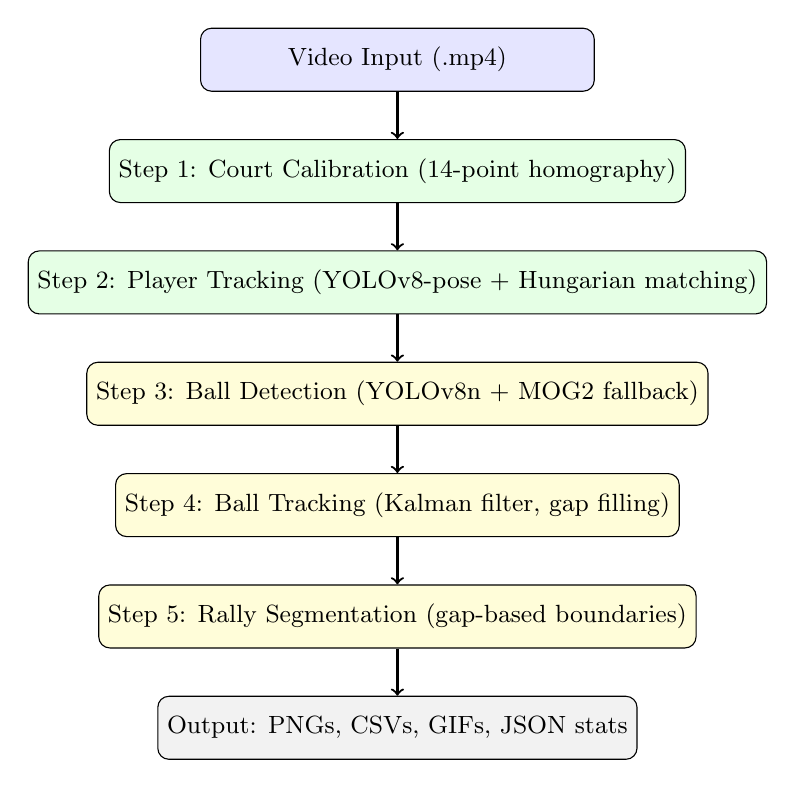
\begin{tikzpicture}[
    node distance=0.6cm,
    box/.style={draw, rounded corners, minimum width=5cm, minimum height=0.8cm,
                text centered, font=\small},
    arrow/.style={->, thick}
]
\node[box, fill=blue!10]  (input)   {Video Input (.mp4)};
\node[box, fill=green!10, below=of input]  (calib)   {Step 1: Court Calibration (14-point homography)};
\node[box, fill=green!10, below=of calib]  (player)  {Step 2: Player Tracking (YOLOv8-pose + Hungarian matching)};
\node[box, fill=yellow!15, below=of player] (ball)    {Step 3: Ball Detection (YOLOv8n + MOG2 fallback)};
\node[box, fill=yellow!15, below=of ball]   (kalman)  {Step 4: Ball Tracking (Kalman filter, gap filling)};
\node[box, fill=yellow!15, below=of kalman] (rally)   {Step 5: Rally Segmentation (gap-based boundaries)};
\node[box, fill=gray!10,  below=of rally]   (output)  {Output: PNGs, CSVs, GIFs, JSON stats};

\draw[arrow] (input)  -- (calib);
\draw[arrow] (calib)  -- (player);
\draw[arrow] (player) -- (ball);
\draw[arrow] (ball)   -- (kalman);
\draw[arrow] (kalman) -- (rally);
\draw[arrow] (rally)  -- (output);
\end{tikzpicture}
\end{center}

Steps 1--2 are reliable and run in production. Steps 3--5 are implemented but blocked by ball detection accuracy.

% ─────────────────────────────────────────────────────────────────────────────
\section{Completed Work}

\subsection{Court Calibration}

A 14-point click calibration UI allows the user to mark known court landmarks on the first frame of a video. These are mapped to real-world court coordinates (in metres) using OpenCV's \texttt{findHomography}. The resulting $3\times3$ matrix is cached to disk (\texttt{assets/homography.npy}) and reused on subsequent runs unless \texttt{--calibrate} is passed.

This homography is used throughout the pipeline to convert pixel coordinates to court-space positions, enabling all distance and speed calculations to be in metres rather than pixels.

\subsection{Player Tracking}

\textbf{Current approach (Day~12, default):} YOLOv8n-pose runs full-frame inference on every video frame. The two highest-confidence person detections are extracted. A cost matrix is built from Euclidean distance in pixel space, and the Hungarian algorithm (via \texttt{scipy.optimize.linear\_sum\_assignment}) assigns detections to Player~1 and Player~2, maintaining consistent identities across frames.

Ground positions are derived from pose keypoints using a three-tier fallback:
\begin{enumerate}
    \item Ankle midpoint (COCO keypoints 15 \& 16) — preferred
    \item Knee midpoint (keypoints 13 \& 14) — if ankles not visible
    \item Hip midpoint (keypoints 11 \& 12) — final fallback
\end{enumerate}

\textbf{Legacy approach:} A MediaPipe-based tracker crops the frame into top and bottom halves before running pose estimation. This approach is retained for comparison but is prone to identity swaps when players are close together, and the hip-only fallback introduces a systematic $\sim$1\,m upward bias in the Y-position estimate.

\textbf{Known limitation:} Player initialisation (assigning which detection is P1 vs P2) relies on vertical position in the first frame. If both players appear on the same half of the court initially, assignment is incorrect and persists for the entire clip.

Figure~\ref{fig:pixel} shows the tracked player positions overlaid directly on the video frame, and Figure~\ref{fig:court} shows the same trajectories projected into court space via the homography.

\begin{figure}[H]
    \centering
    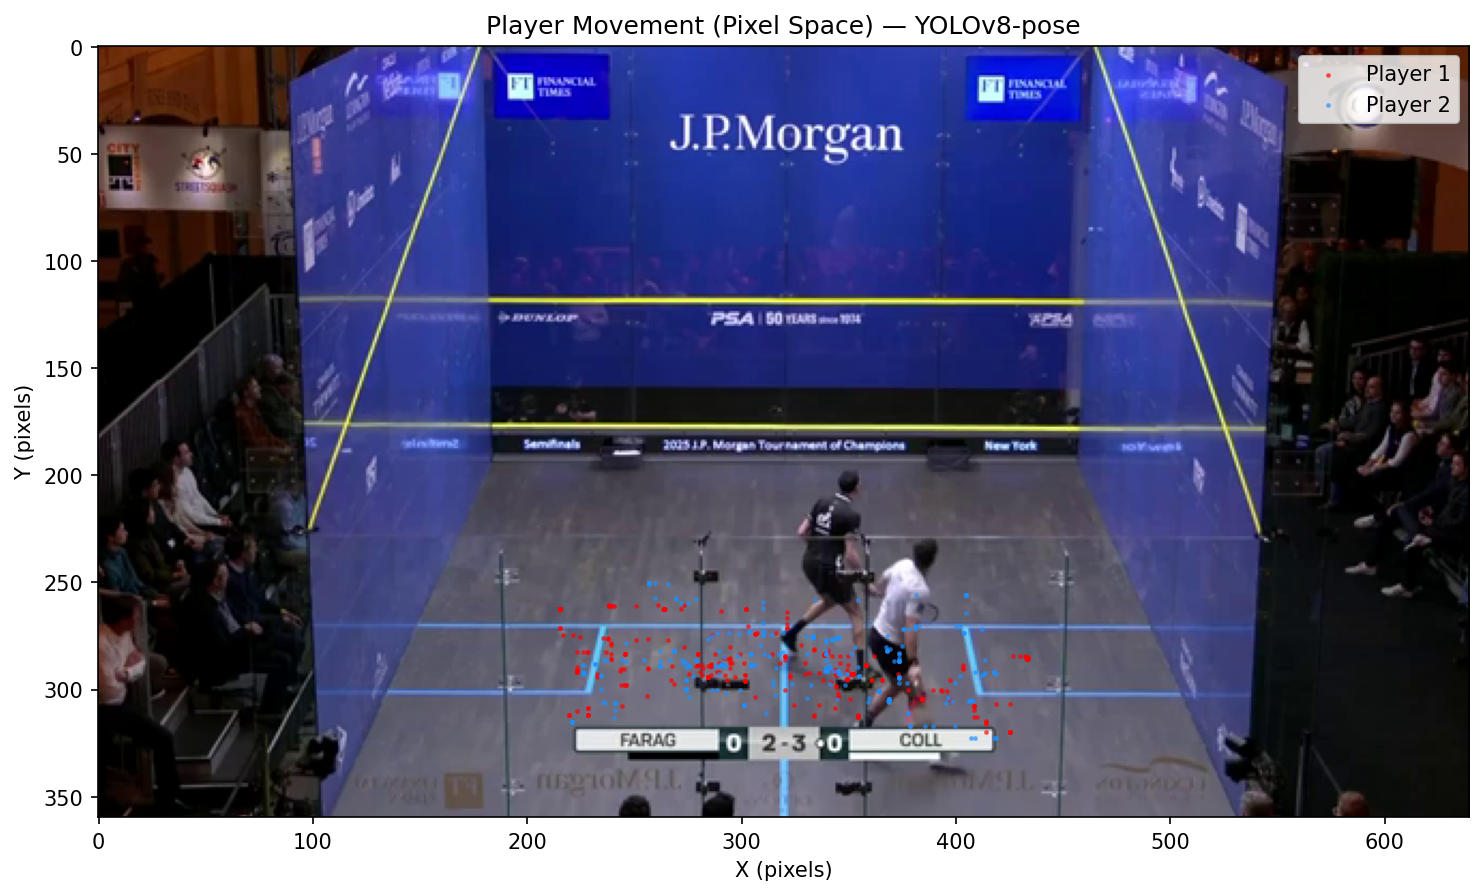
\includegraphics[width=\linewidth]{pixel_positions.png}
    \caption{Player movement in pixel space overlaid on the match video. Red dots = Player~1, blue dots = Player~2. The yellow lines show the calibrated court boundary used for the homography.}
    \label{fig:pixel}
\end{figure}

\begin{figure}[H]
    \centering
    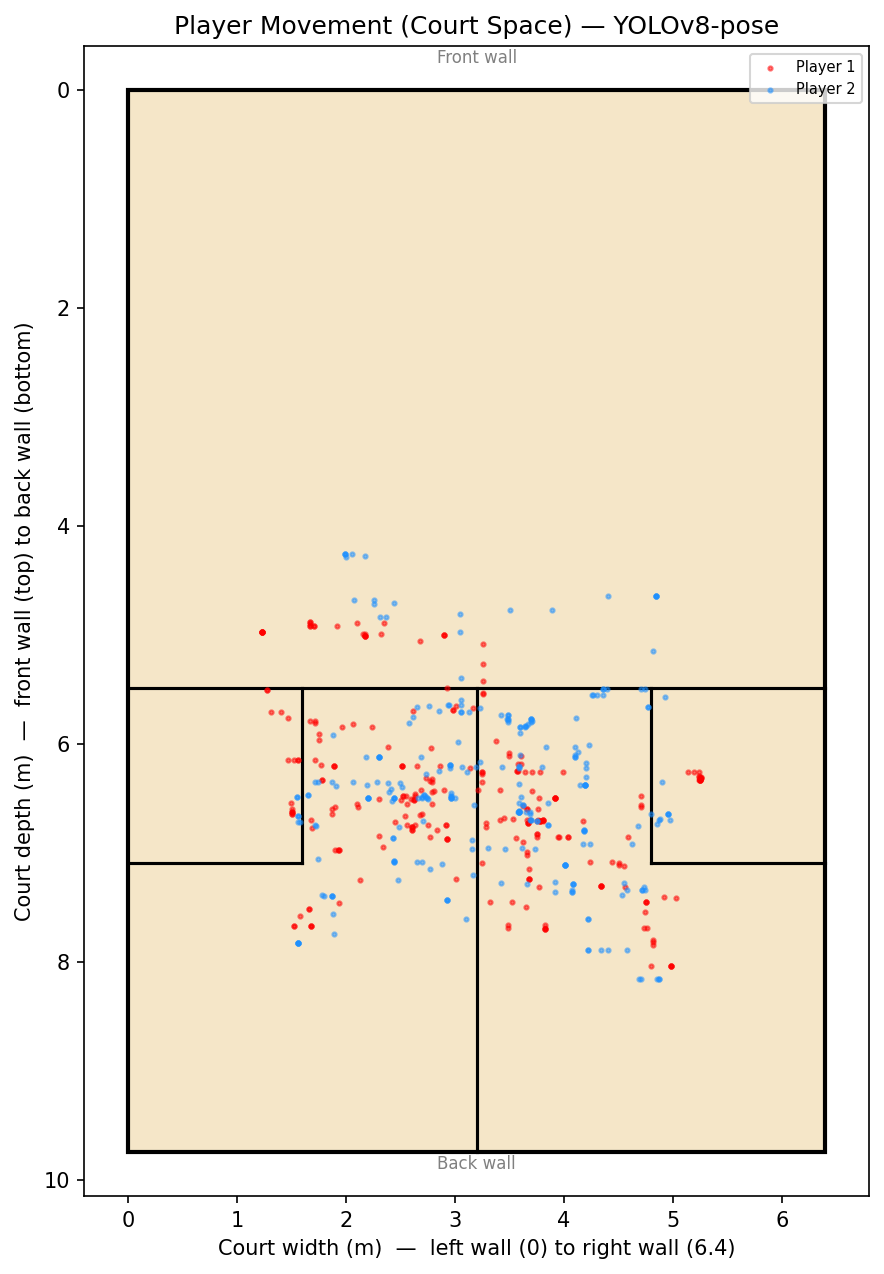
\includegraphics[width=0.6\linewidth]{court_positions.png}
    \caption{Player trajectories projected into court space (metres). Each dot is one frame. The court diagram is drawn to scale: 9.75\,m deep $\times$ 6.4\,m wide.}
    \label{fig:court}
\end{figure}

\subsection{Player Heatmaps}

Gaussian kernel density estimation is applied to the court-space position sequence for each player, producing a smooth heatmap that shows where each player spends the most time. Figure~\ref{fig:heatmaps} shows the resulting heatmaps side by side.

\begin{figure}[H]
    \centering
    \begin{subfigure}[t]{0.48\linewidth}
        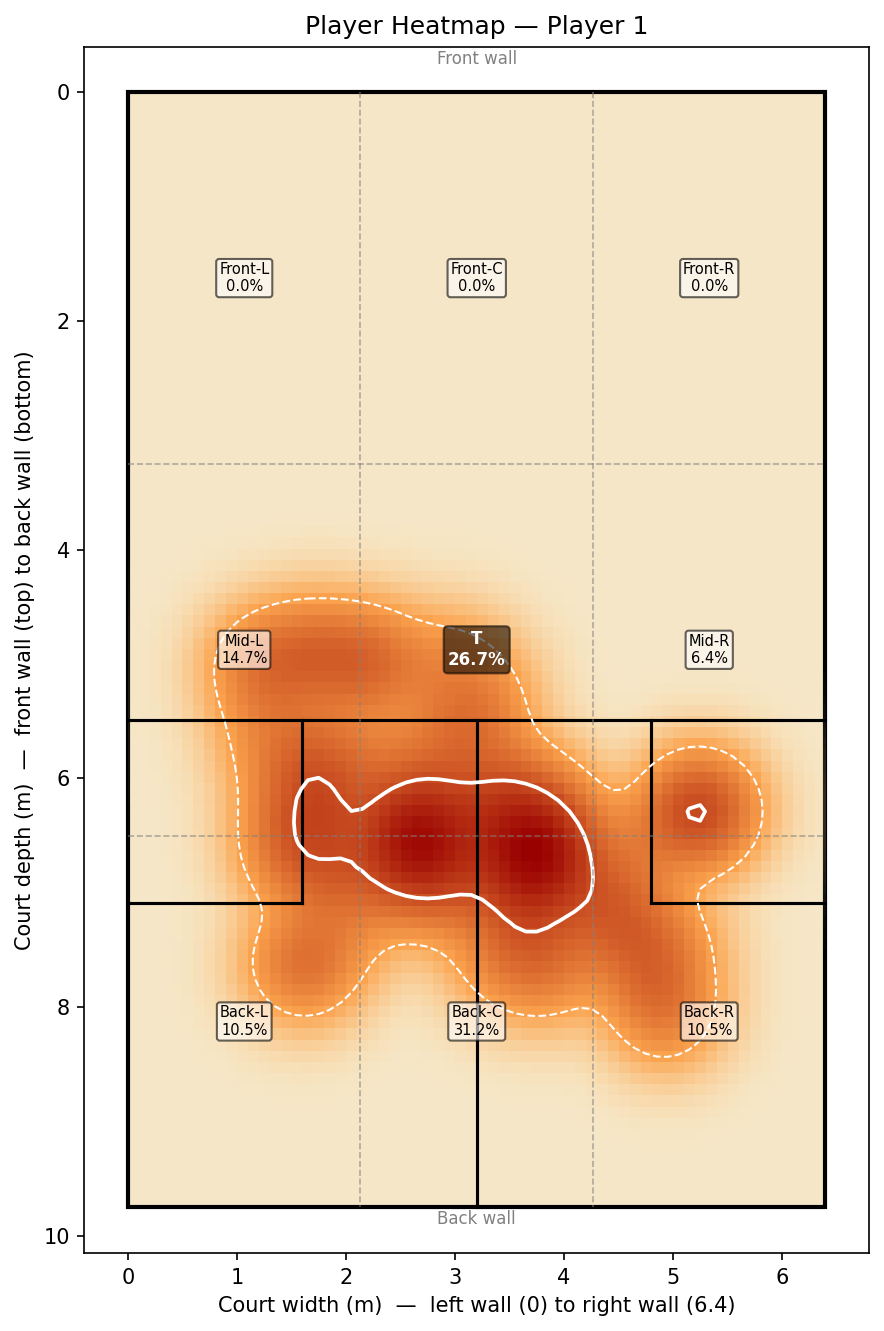
\includegraphics[width=\linewidth]{heatmap_player1.png}
        \caption{Player 1 — concentrated around back-centre and the T.}
    \end{subfigure}
    \hfill
    \begin{subfigure}[t]{0.48\linewidth}
        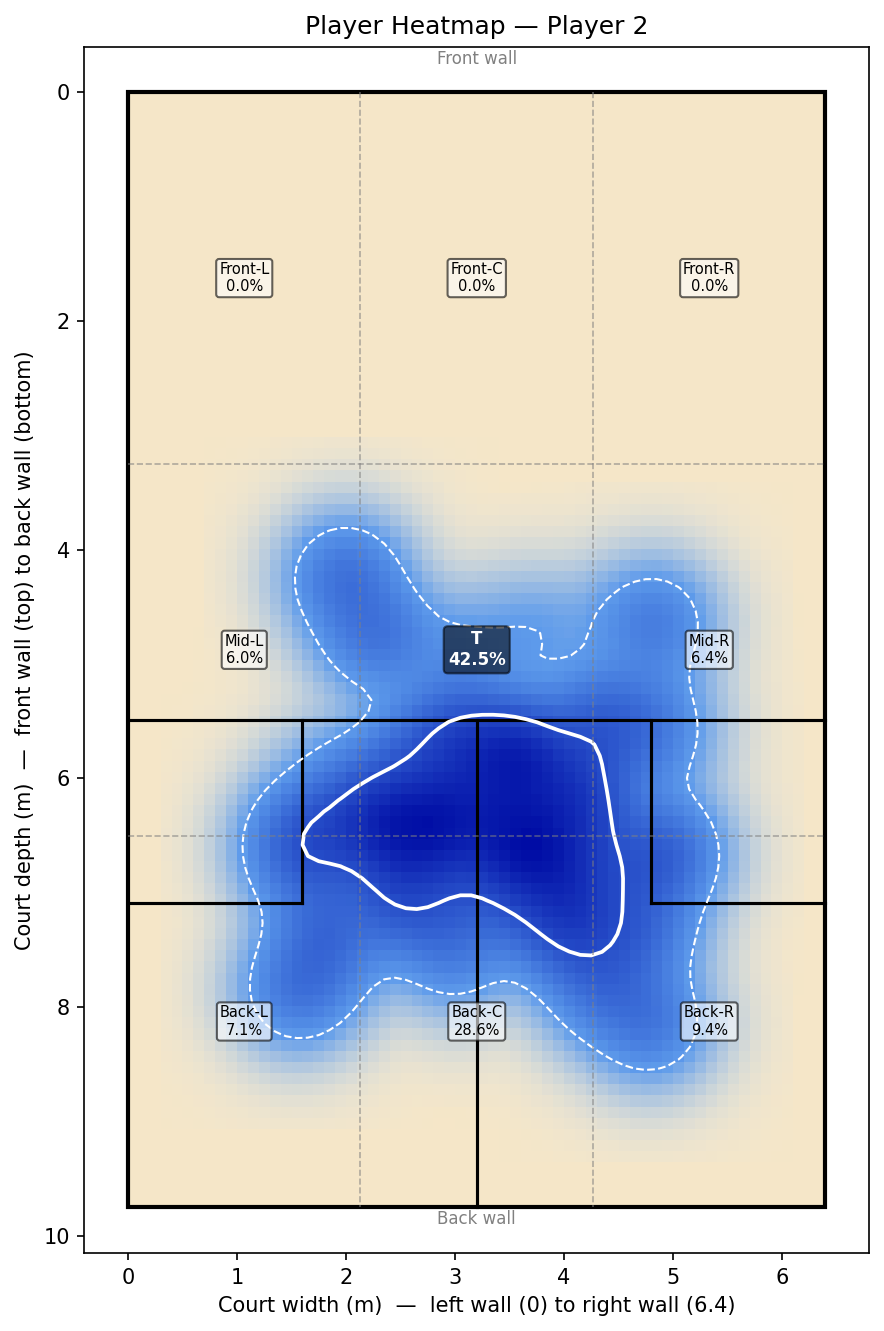
\includegraphics[width=\linewidth]{heatmap_player2.png}
        \caption{Player 2 — tighter concentration around the T zone.}
    \end{subfigure}
    \caption{Gaussian heatmaps for both players. Warmer colours indicate more time spent in that region. The T junction is marked with a white label.}
    \label{fig:heatmaps}
\end{figure}

\subsection{Zone Breakdown}

The court is divided into a $3 \times 3$ grid (Front/Mid/Back $\times$ Left/Centre/Right), matching standard squash tactical analysis zones. The fraction of time each player spends in each zone is computed and displayed as a percentage. Figure~\ref{fig:zones} shows the zone breakdown for the analysed clip.

\begin{figure}[H]
    \centering
    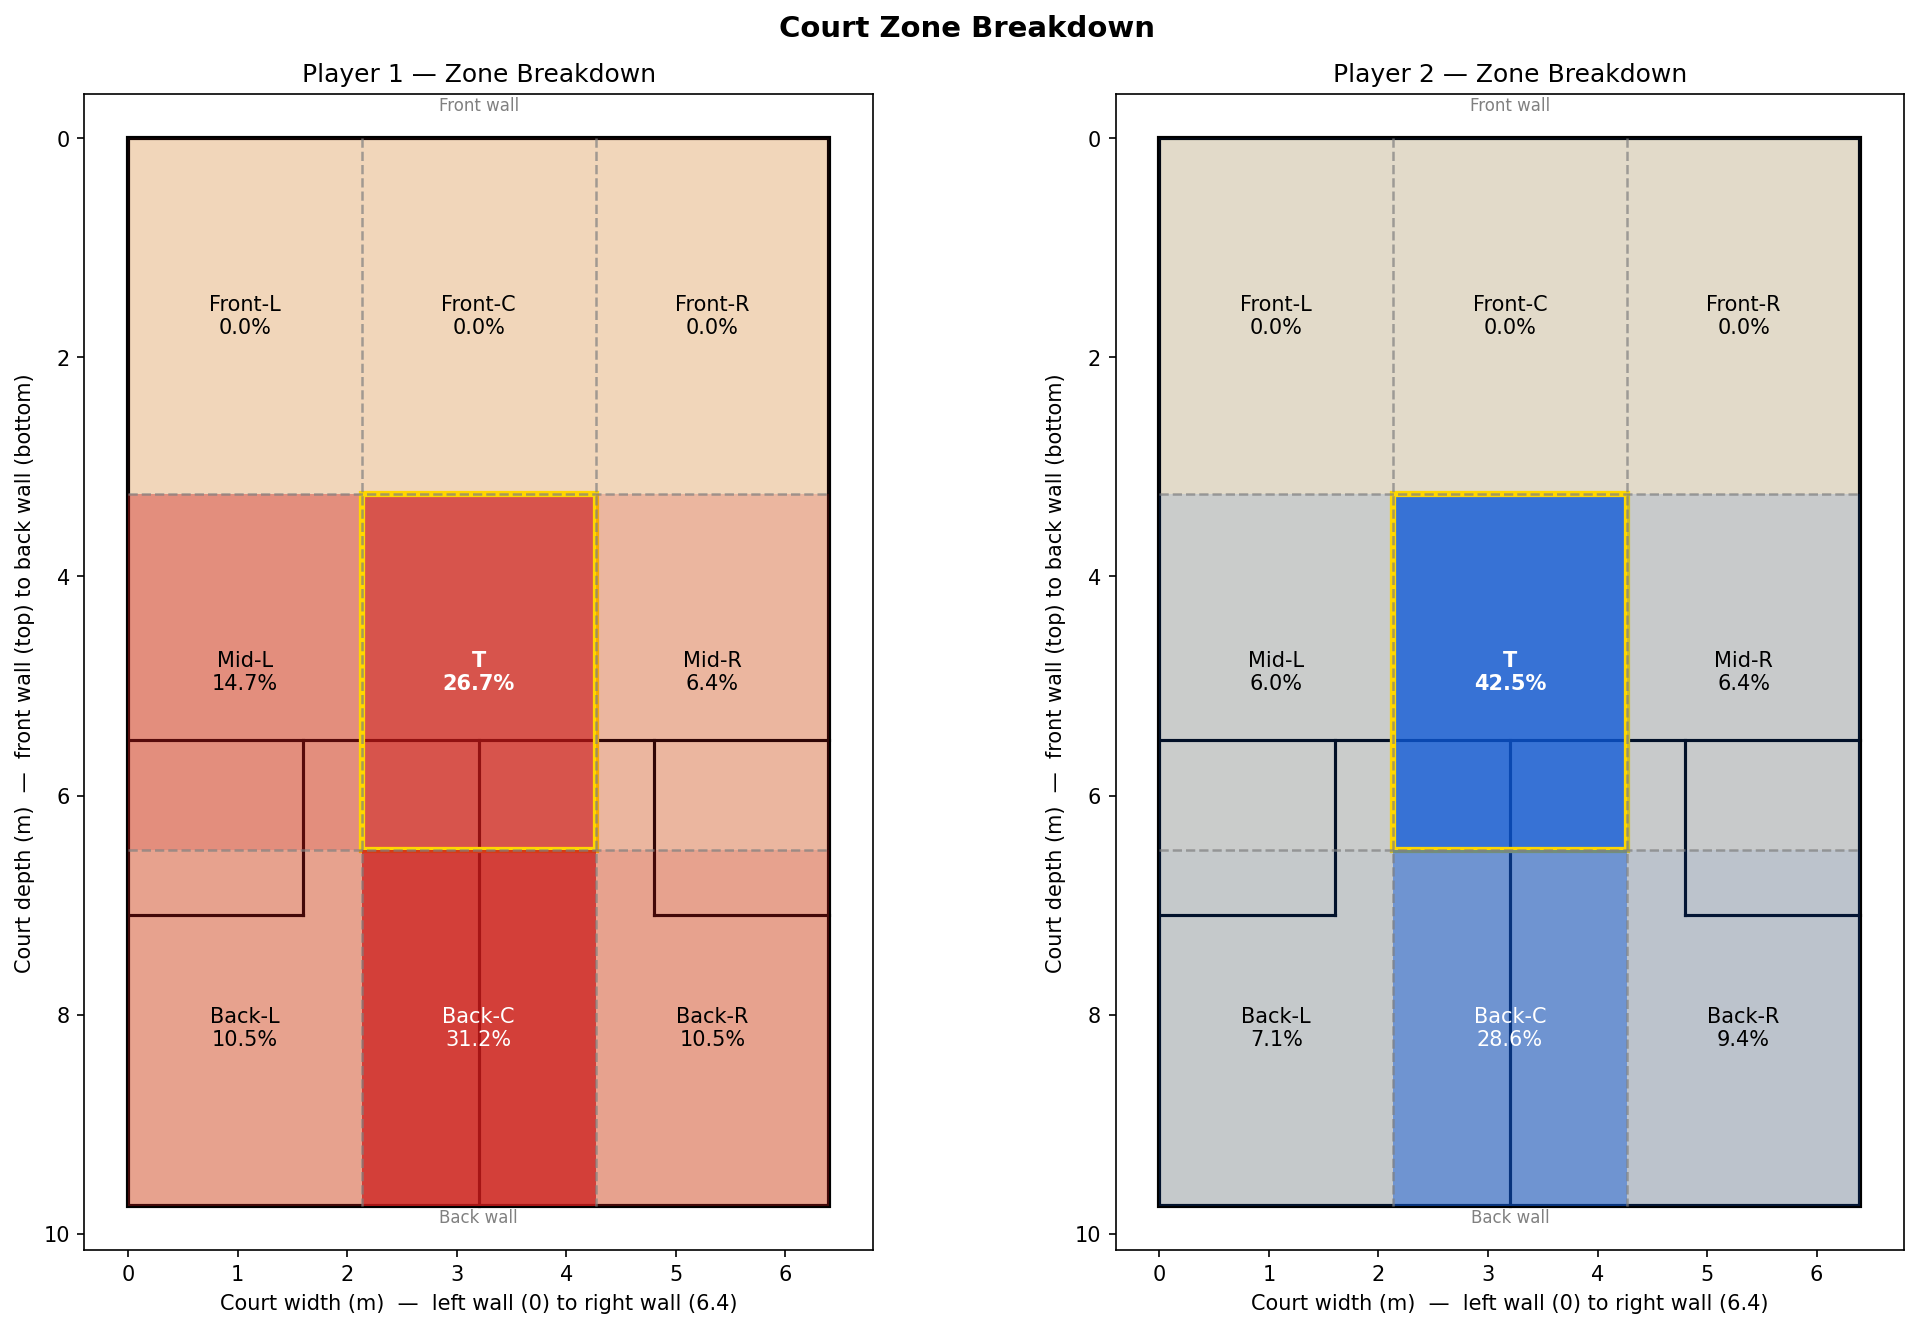
\includegraphics[width=\linewidth]{zone_breakdown.png}
    \caption{Zone-by-zone court coverage for each player. The T zone (centre of mid-court) is highlighted in gold. Player~1 spent 26.7\% of the clip on the T; Player~2 spent 42.5\%.}
    \label{fig:zones}
\end{figure}

\subsection{Movement Statistics}

The following per-player statistics are computed from court-space position sequences:

\begin{center}
\begin{tabular}{lll}
\toprule
\textbf{Metric} & \textbf{Method} & \textbf{Unit} \\
\midrule
Total distance & Sum of frame-to-frame Euclidean distances & m \\
Average speed & Total distance / clip duration & m/s \\
Peak speed & 95th percentile of instantaneous speeds & m/s \\
T-position time & \% of frames within 1.25\,m of T junction & \% \\
Front/back split & Fraction of positions with $y < 5.5$\,m (mid-court) & \% \\
\bottomrule
\end{tabular}
\end{center}

Figure~\ref{fig:timeseries} shows three time-series analytics plots: instantaneous speed, distance from the T, and court depth over the duration of the clip. Figure~\ref{fig:histograms} shows the marginal position distributions for both players.

\begin{figure}[H]
    \centering
    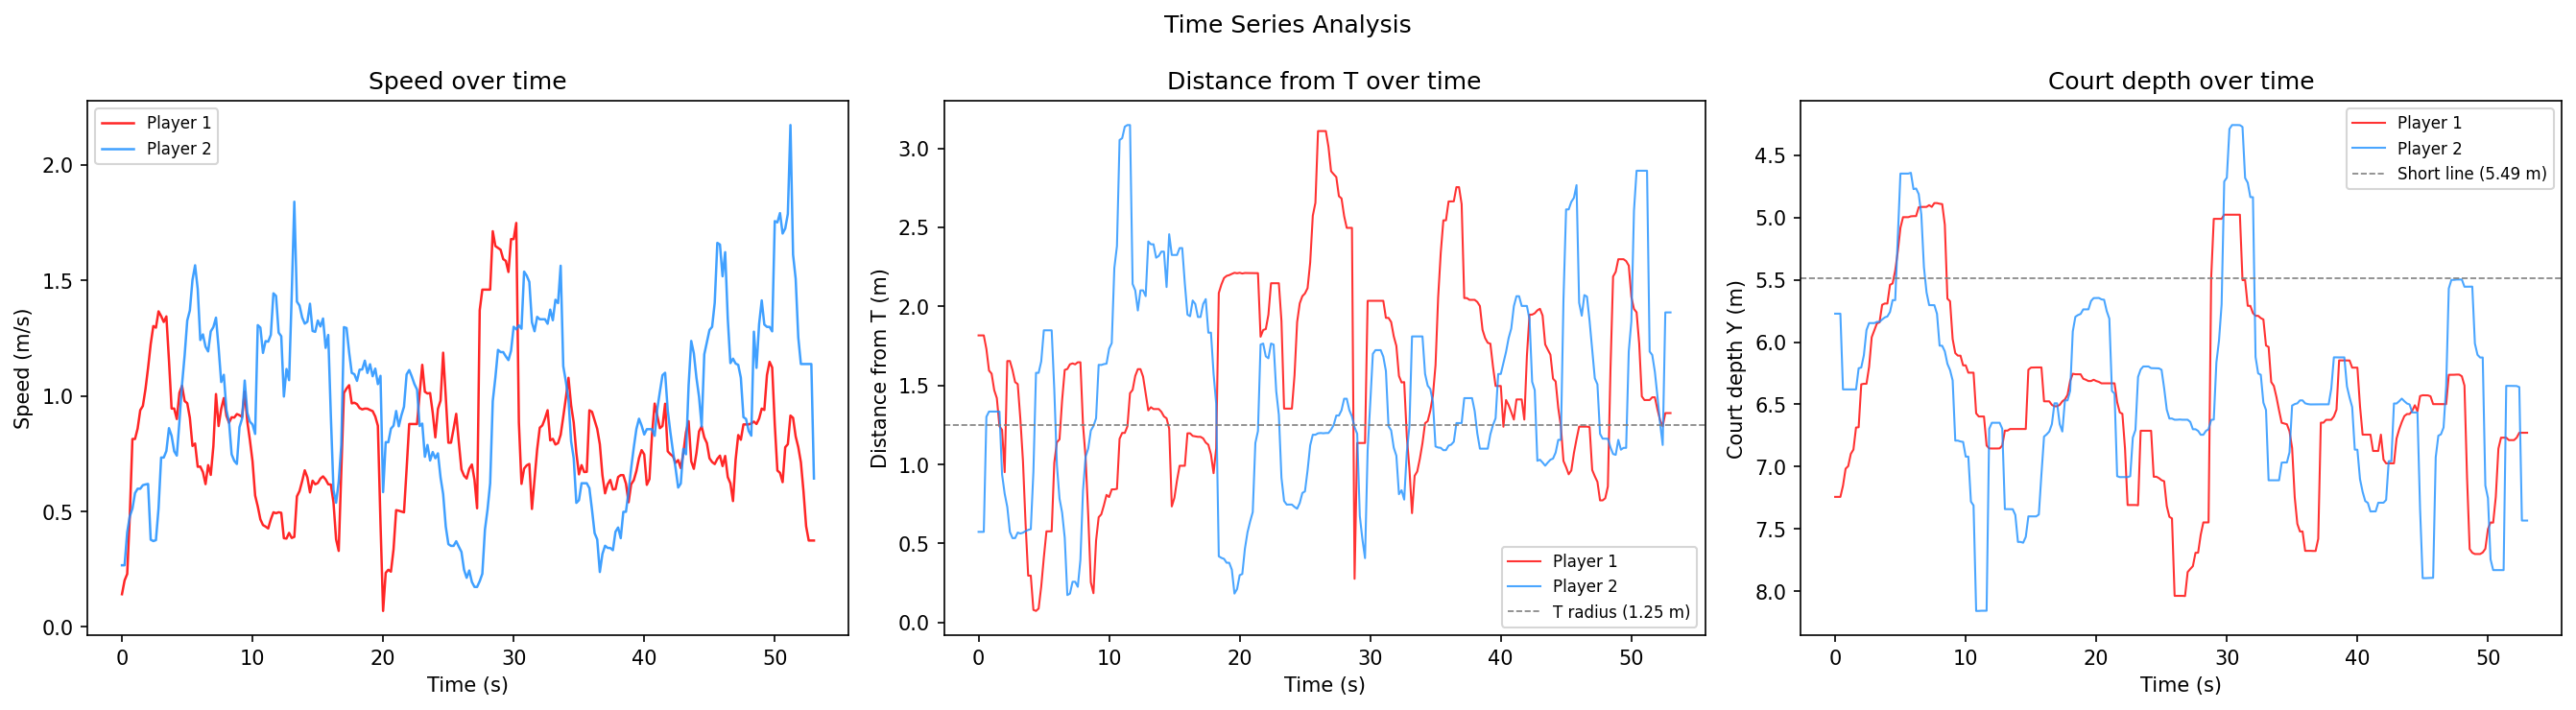
\includegraphics[width=\linewidth]{timeseries.png}
    \caption{Time-series analytics. \textit{Left:} instantaneous speed (m/s). \textit{Centre:} distance from the T junction (m); the grey dashed line marks the 1.25\,m T-proximity threshold. \textit{Right:} court depth over time (m); the horizontal line at 5.49\,m marks the short line.}
    \label{fig:timeseries}
\end{figure}

\begin{figure}[H]
    \centering
    
\includegraphics[width=\linewidth]{histograms.png}
    \caption{Marginal position distributions for both players. \textit{Left:} court depth (Y axis); both players cluster around 6--7\,m (back-court), consistent with the zone breakdown. \textit{Right:} lateral position (X axis); both players centre around 3\,m (court midline), as expected.}
    \label{fig:histograms}
\end{figure}

\subsection{Testing}

A \texttt{pytest} test suite covers the major pipeline components:

\begin{center}
\begin{tabular}{ll}
\toprule
\textbf{Test file} & \textbf{What it validates} \\
\midrule
\texttt{test\_tracking.py} & Player tracking frame-to-frame consistency \\
\texttt{test\_homography.py} & Calibration point reprojection accuracy \\
\texttt{test\_stats.py} & Distance/speed computation correctness \\
\texttt{test\_zones.py} & Zone assignment logic \\
\texttt{test\_timeseries.py} & Time-series analytics \\
\texttt{test\_plots.py} & Visualisation output (file existence, format) \\
\texttt{test\_validate.py} & Ground-truth validation helpers \\
\bottomrule
\end{tabular}
\end{center}

% ─────────────────────────────────────────────────────────────────────────────
\section{In-Progress Work}

\subsection{Ball Detection}

Ball detection uses a two-stage approach:

\begin{enumerate}
    \item \textbf{YOLOv8n (COCO class 32, ``sports ball'')} runs full-frame inference. COCO training data does not include squash balls (black, $\sim$40\,mm diameter), so recall is low.
    \item \textbf{MOG2 background subtraction} detects foreground blobs, which are filtered by circularity and size to identify ball candidates. This catches fast-moving balls that YOLO misses.
\end{enumerate}

When both methods fire, YOLO is preferred if its detection falls within 60 pixels of the MOG2 candidate; otherwise MOG2 is used.

\textbf{Current recall estimate: $\sim$60--70\%.} The target is $\geq$70\% on a labelled test set (not yet assembled). At 25\,fps, a hard-driven ball ($\sim$150\,km/h) travels $\sim$1.67\,m per frame, making any frame-skip approach non-viable.

\subsection{Ball Tracking (Kalman Filter)}

A 4-state Kalman filter ($x, y, v_x, v_y$) smooths the raw detection sequence and fills gaps up to 5 consecutive missed frames using constant-velocity prediction. Gaps longer than 5 frames are logged as ``ball lost'' segments. The smoothed output is saved separately from the raw detections.

Figure~\ref{fig:ball} shows the current state of ball tracking on the analysed clip. Only 3 detections were successfully located, illustrating the severity of the ball detection problem.

\begin{figure}[H]
    \centering
    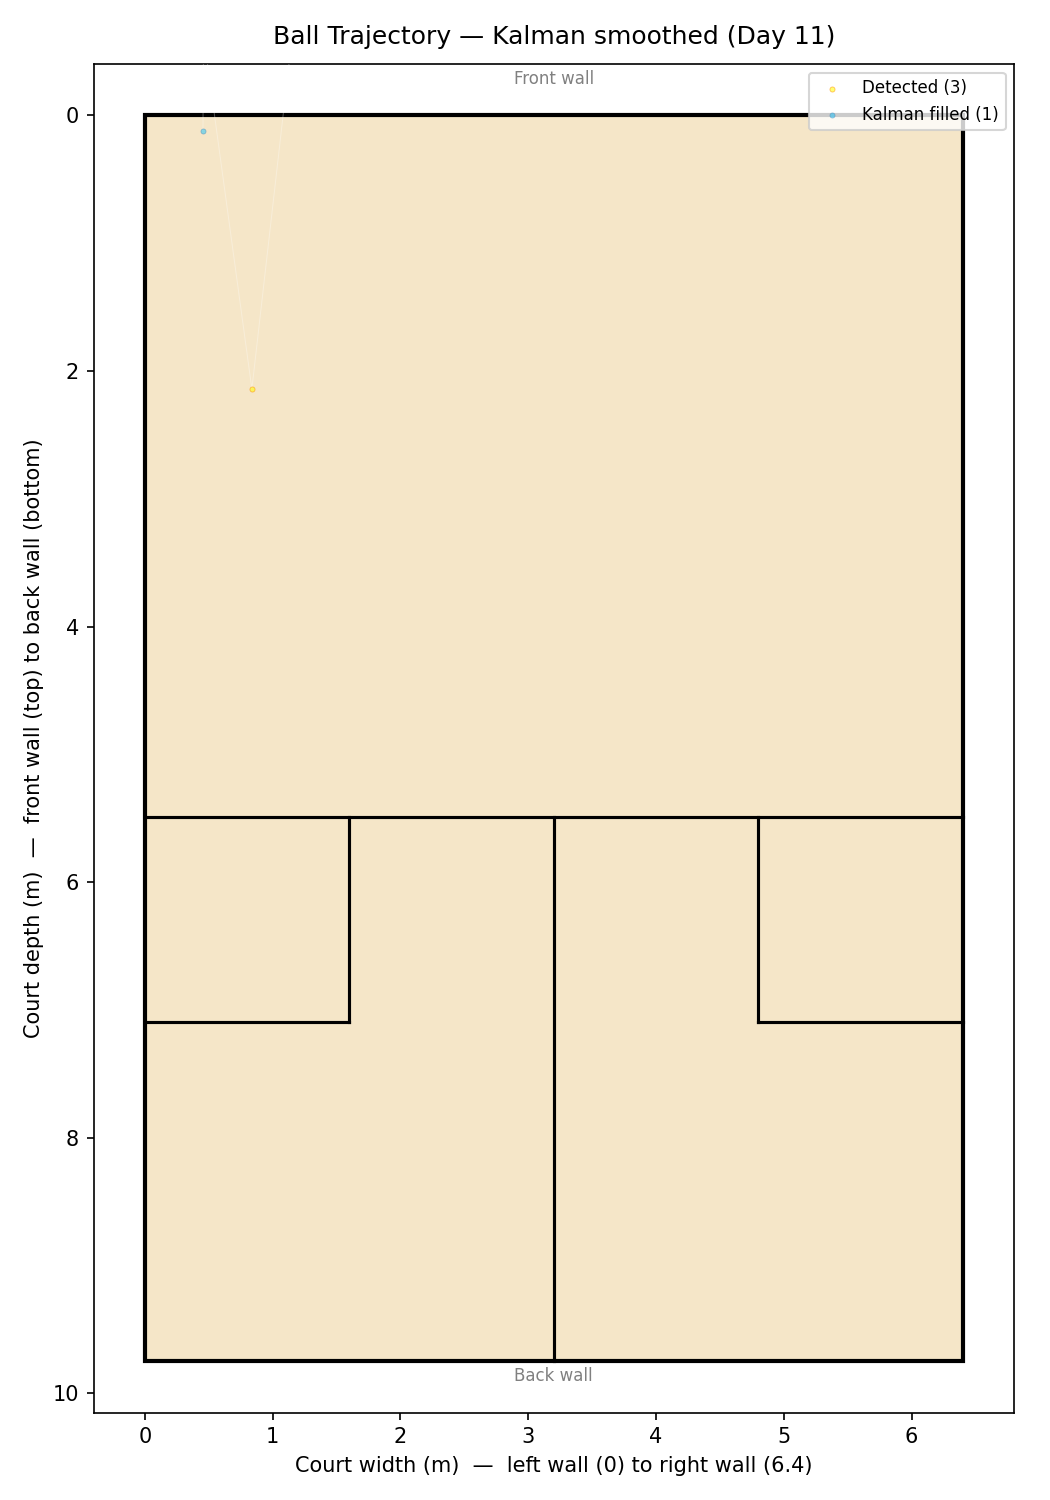
\includegraphics[width=0.65\linewidth]{ball_trajectory_smooth.png}
    \caption{Kalman-smoothed ball trajectory for the analysed clip. Yellow dots are YOLO/MOG2 detections; the blue dot is a Kalman-filled position. Only 3 positions were detected across the entire clip, demonstrating that ball tracking is the primary current blocker.}
    \label{fig:ball}
\end{figure}

\subsection{TrackNetV4 (Experimental)}

A custom implementation of the TrackNetV4 architecture has been trained as an alternative ball detector. The model is a U-Net with a motion prompt layer. Inputs are 11 channels: 3 consecutive RGB frames plus 2 inter-frame difference maps. The output is a 3-channel heatmap (one Gaussian blob per input frame indicating the ball position).

\textbf{Status:} The model has been trained on labelled frames from the match video, but inference quality is poor. Ball detections are noisy and unreliable. This remains an active area of investigation.

\subsection{Rally Segmentation}

Rally boundaries are detected by finding gaps in the ball-detection sequence longer than 20 frames ($\sim$0.8\,s at 25\,fps). For each rally, the following are computed:
\begin{itemize}
    \item Start and end frame numbers
    \item Duration in seconds
    \item Approximate shot count (velocity direction reversals in ball trajectory)
    \item Per-player distance covered during the rally
\end{itemize}

Because rally segmentation depends on ball detection, the output is unreliable at current detection recall levels. Figure~\ref{fig:rally_timeline} shows the rally timeline detected from the current clip, and Figure~\ref{fig:combined} shows both player trajectories and ball detections coloured by rally.

\begin{figure}[H]
    \centering
    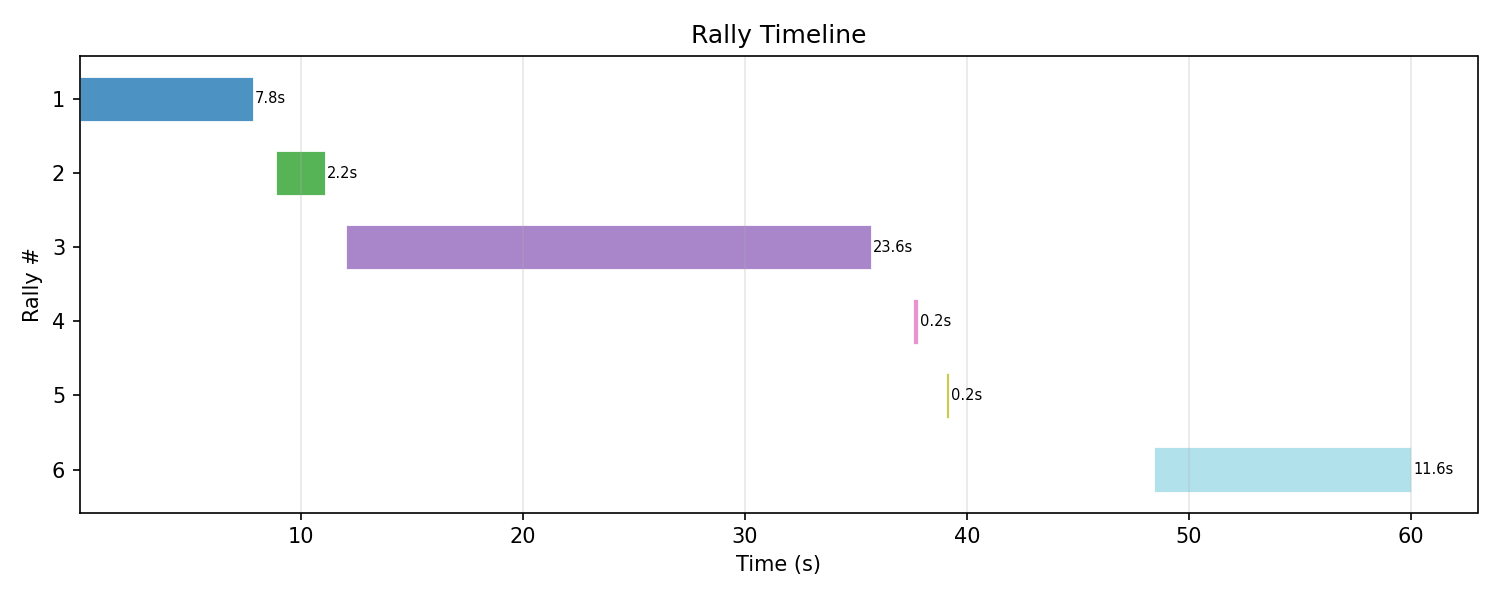
\includegraphics[width=\linewidth]{rally_timeline.png}
    \caption{Detected rally timeline. Six rallies were segmented, ranging from 0.2\,s to 23.6\,s. The very short rallies (0.2\,s) are likely artefacts of the low ball detection recall rather than real rallies.}
    \label{fig:rally_timeline}
\end{figure}

\begin{figure}[H]
    \centering
    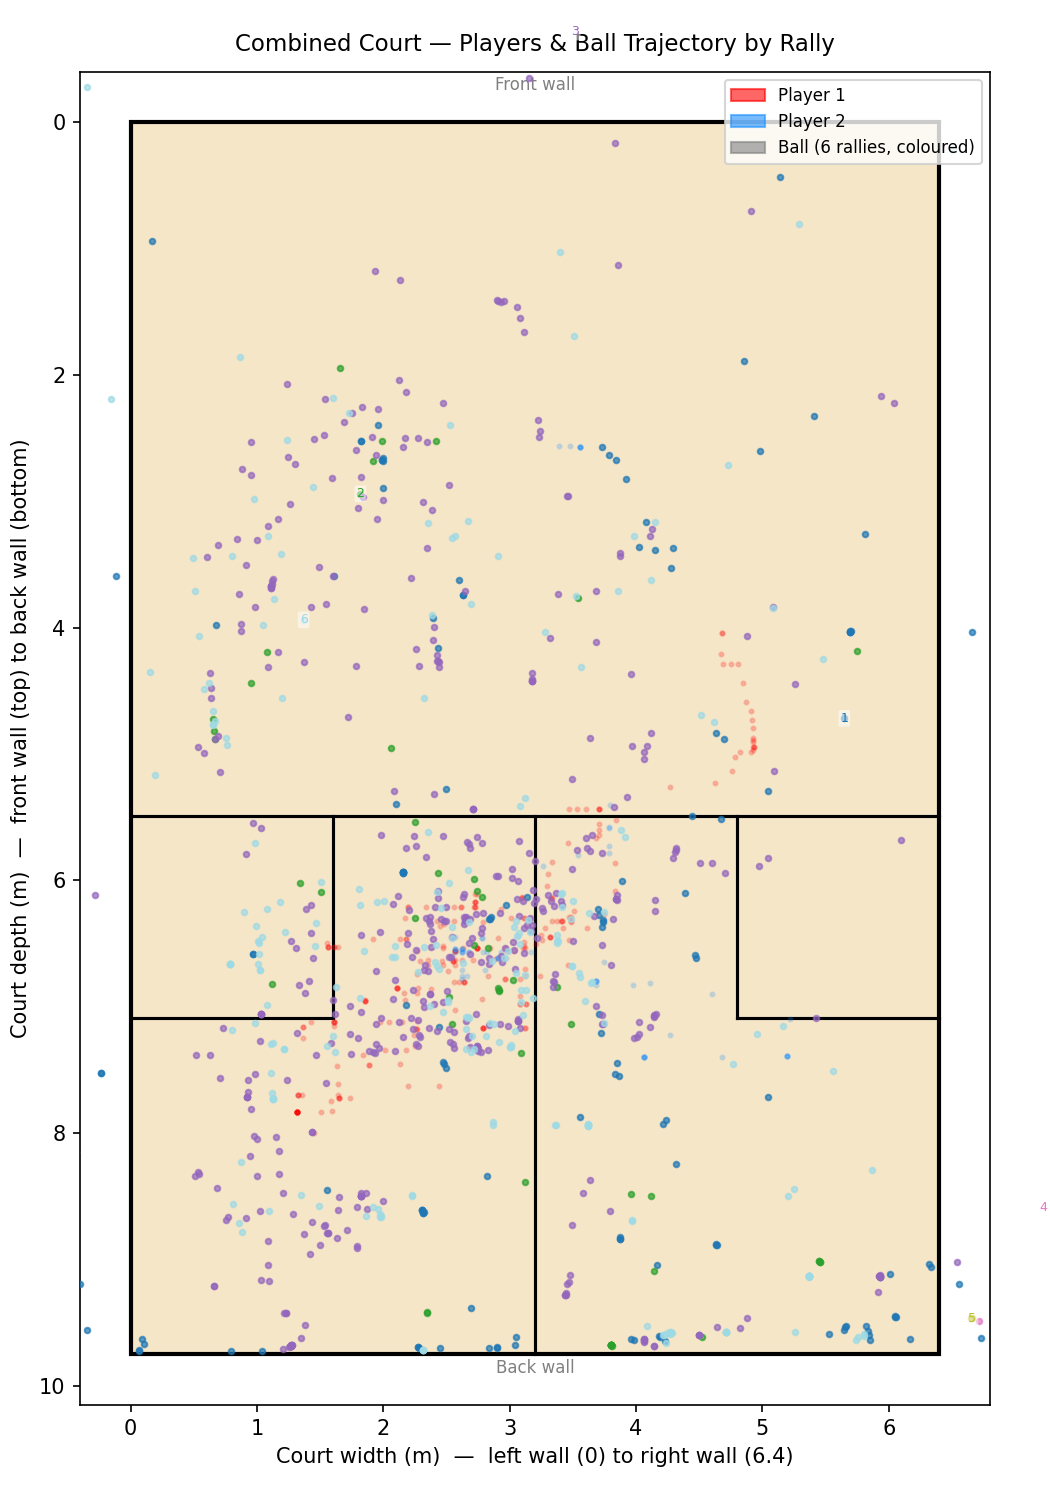
\includegraphics[width=0.65\linewidth]{combined_court.png}
    \caption{Combined court diagram showing Player~1 (red), Player~2 (blue), and ball detections (coloured by rally). The sparse ball detections across the court highlight the detection gap that needs to be resolved.}
    \label{fig:combined}
\end{figure}

% ─────────────────────────────────────────────────────────────────────────────
\section{Known Issues \& Blockers}

\begin{center}
\begin{tabular}{p{4cm}p{7cm}l}
\toprule
\textbf{Issue} & \textbf{Description} & \textbf{Severity} \\
\midrule
Ball detection recall & $\sim$60--70\%, target $\geq$70\%. Squash balls absent from COCO training data. TrackNetV4 trained but not working reliably. & \blocked{High} \\[6pt]
Player initialisation & If both players are in the same half of the court on frame~1, P1/P2 assignment is incorrect for the entire clip. & \inprogress{Medium} \\[6pt]
Identity swap & No automatic recovery from identity swaps (proximity warning exists but no correction). & \inprogress{Medium} \\[6pt]
Per-rally stats & Stats are computed per-clip; per-rally breakdowns are planned but not yet implemented. & Low \\[6pt]
Manual calibration & 14-point click UI takes 3--5 minutes per court setup; error-prone on low-resolution footage. & Low \\[6pt]
Stats persistence & Match history stored as a flat JSON file; SQLite migration planned but not done. & Low \\
\bottomrule
\end{tabular}
\end{center}

% ─────────────────────────────────────────────────────────────────────────────
\section{Remaining Planned Work}

\subsection*{Week 3 — Web Interface}
\begin{itemize}[noitemsep]
    \item Streamlit dashboard for video upload and results display
    \item In-browser court calibration (click on video frame)
    \item PDF report export
    \item Match history and player profiles
\end{itemize}

\subsection*{Week 4 — Ball Tracking \& Rally Intelligence}
\begin{itemize}[noitemsep]
    \item Resolve ball detection recall ($\geq$70\% on labelled test set)
    \item Assemble and label ball detection ground truth dataset
    \item Fine-tune or replace detection approach (TrackNetV4 or domain-specific model)
    \item Shot classification (serve, drive, drop, boast, lob) from ball trajectory
    \item Front wall heatmap
    \item Automatic video highlight clips
\end{itemize}

\subsection*{Week 5 — Shot Outcomes \& Deployment}
\begin{itemize}[noitemsep]
    \item Shot outcome mapping (winner, error, let)
    \item Momentum analysis (rolling rally win rates)
    \item End-to-end accuracy report (player position RMSE, ball F1, rally F1)
    \item Docker container for portable deployment
    \item Physics-based ball model (UKF with gravity/drag)
\end{itemize}

% ─────────────────────────────────────────────────────────────────────────────
\section{Technical Stack}

\begin{center}
\begin{tabular}{ll}
\toprule
\textbf{Library} & \textbf{Purpose} \\
\midrule
OpenCV & Video I/O, background subtraction, homography \\
Ultralytics (YOLOv8) & Person detection, pose estimation, sports-ball detection \\
MediaPipe & Legacy pose estimation (kept for comparison) \\
NumPy / SciPy & Numerical processing, Hungarian assignment, Kalman filter \\
PyTorch & TrackNetV4 model training and inference \\
Matplotlib & All visualisations \\
pytest & Automated testing \\
\bottomrule
\end{tabular}
\end{center}

% ─────────────────────────────────────────────────────────────────────────────
\section{Summary}

The first two weeks of development have produced a functional player-tracking and statistics pipeline. Court calibration, YOLOv8-pose based tracking, movement metrics, zone breakdowns, and heatmap visualisations all work reliably and are covered by automated tests.

The main current challenge is ball tracking. The squash ball is small, fast, dark, and not well-represented in standard computer vision datasets. Two approaches have been attempted (YOLO+MOG2 and a custom TrackNetV4 implementation); neither yet meets the quality threshold needed to unlock the downstream rally and shot analysis features.

Once ball detection is resolved, the path to a complete match analysis report --- covering player movement, rally-by-rally statistics, shot classification, and front wall tendencies --- is straightforward.

\end{document}
